\documentclass[11pt]{article}

\usepackage[margin=1in]{geometry}
\usepackage{amsmath,amssymb}
\usepackage{graphicx}
\usepackage{booktabs}
\usepackage{hyperref}
\usepackage{xcolor}
\usepackage{caption}
\usepackage{natbib}

\hypersetup{colorlinks=true, linkcolor=blue, citecolor=blue, urlcolor=blue}

% Central place for all YouTube video links referenced in the paper.
% Fill in each \def with the real YouTube URL after uploading
% three_body/manim/final/*.mp4, then just recompile -- nothing else in
% main.tex needs to change.

% Scene A: the validated figure-eight orbit (three_body/manim/final/scene_a_figure_eight_orbit_with_music.mp4)
\def\videoFigureEight{https://youtu.be/uMNLTKFUXI4}

% Scene B: hierarchical stability, stable vs disrupted (three_body/manim/final/scene_b_hierarchical_stability_with_music.mp4)
% (re-rendered to fix camera-tracking clipping bug -- see notes.md)
\def\videoHierarchical{https://youtu.be/VID2Qx_FtoE}

% Scene C: escape/collision statistics (three_body/manim/final/scene_c_survival_statistics_with_music.mp4)
% (re-rendered to fix camera-tracking clipping bug -- see notes.md)
\def\videoSurvival{https://youtu.be/Zm_S9v5XTLs}


\newcommand{\watch}[2]{\href{#1}{\textcolor{blue}{\textit{[watch: #2]}}}}

\title{Periodic Orbits and Finite-Time Stability\\
in the Gravitational Three-Body Problem:\\
\large A Computational Investigation}
\author{Aditya Bhattacharjee}
\date{\today}

\begin{document}
\maketitle

\begin{abstract}
Newton's equations for the three-body problem have no general formula for a
solution. But a computer can build one specific solution and check that it
is correct to very high precision. This paper asks two questions about what
a computed solution can actually promise. First: if we do not start from
any orbit we already know, can a search still find a brand-new periodic
orbit -- one that retraces the exact same path forever? Second: if we pick
a length of time $T$, can we build a system that we know, or can at least
show is likely, to survive at least that long without colliding or flying
apart? We built two independent orbit-solvers and checked that they agree
to within $5\times10^{-12}$ over one full orbit. Using them, we re-derived
the well-known figure-eight orbit and confirmed it to $10^{-12}$ precision.
We then tried four different from-scratch searches for new periodic
orbits. All four failed to find one within a reasonable amount of
computing time -- but the reason they failed is itself the interesting
result. Without angular momentum, nothing stops the three bodies from
colliding, so most of the starting points we searched land near a
collision instead of near a stable orbit. This helps explain why past
researchers needed much more computing power, or a smarter search method,
to succeed where a simple search does not. For the second question, we
found two separate ways to build a system that survives a chosen amount of
time. One is a formula (Mardling \& Aarseth, 2001) for a tight pair of
stars orbited by a third, distant star: if the outer orbit is wide enough,
the system stays stable, and we confirmed this by simulating it for 500
orbits. The other is statistical: out of 200 randomly generated three-body
systems, we measured what fraction survived at least $T$ time units, for
several values of $T$. Three short animations, built from this same
simulation data, accompany the paper.
\end{abstract}

\tableofcontents

% ======================================================================
\section{Introduction}
% ======================================================================

Newton's law of gravity gives an exact equation of motion for any number of
masses. But in 1890 Poincar\'e proved that for three or more bodies, this
equation cannot be solved with one general formula built out of ordinary
functions \cite{ChencinerMontgomery2000}. This is not because the algebra
is hard. It is a deeper fact about the dynamics: with three bodies, the
motion is usually chaotic. A tiny change in the starting position leads to
a completely different outcome later, and the motion never settles into a
simple, repeating pattern.

That does not mean nothing useful can be said. Two specific questions turn
out to be answerable with a computer, and they are the subject of this
paper:

\begin{description}
  \item[Q1.] If we do not use any orbit we already know, can a computer
    search find a new starting condition whose orbit is \emph{exactly
    periodic} -- meaning it retraces the same path in phase space after
    some fixed time?
  \item[Q2.] If we pick a target duration $T$, can we find, or build, a
    starting condition whose orbit is likely, or even guaranteed, to stay
    bound -- no collisions, no bodies flying off to infinity -- for at
    least time $T$? This does not require the orbit to be exactly
    periodic.
\end{description}

Popular descriptions of the three-body problem often blur these two
questions together, talking loosely about orbits that are ``stable
forever'' or ``stable for a while.'' Section~\ref{sec:taxonomy} makes this
distinction precise, because the right answer to Q1 and to Q2 depends on
which of several different technical meanings of ``stable'' is meant.

All the numbers in this paper come from code written for this project
(\texttt{three\_body/research/*.py}) and can be reproduced from the saved
random seeds and starting conditions. Every claim taken from earlier
research is cited and was checked against the original paper, not just
recalled from memory (see Section~\ref{sec:methods} and the bibliography).

% ======================================================================
\section{A taxonomy of ``stable''}
\label{sec:taxonomy}
% ======================================================================

There are four different properties worth telling apart.

\begin{enumerate}
  \item \textbf{Periodic.} The orbit closes exactly:
    $X(T) = X(0)$, or $X(T) = R(\theta)\,X(0)$ for some fixed rotation
    $R(\theta)$, if the orbit only closes once the whole picture is also
    rotated (this happens often in this field). This is a property of one
    single orbit, and a computer can check it to almost any precision.
  \item \textbf{Linearly stable and periodic.} Periodic, and also: a tiny
    nudge to the starting condition does not grow over time. Formally,
    every eigenvalue of the orbit's monodromy matrix -- which describes how
    small nudges evolve after one period -- sits exactly on the unit
    circle. This is the strict meaning of ``stable forever,'' and it is
    rare. Most known periodic three-body orbits are periodic but
    \emph{not} stable in this sense: they are exact solutions for one
    exact starting point, and any tiny error, even the rounding error a
    computer makes, eventually destroys the periodicity. The figure-eight
    orbit (Section~\ref{sec:figure8}) is well known partly because it is
    one of the few orbits that is (weakly) stable in this strict sense.
  \item \textbf{Hierarchically stable.} Not periodic, but bound forever
    for a structural reason: a tight pair of bodies orbited by a third,
    distant body, spaced far enough apart that the third body cannot
    disturb the tight pair. This is the sense of ``stable forever'' that
    matches real astronomy -- most triple star systems that last a long
    time are built this way, rather than sitting on an exact periodic
    orbit.
  \item \textbf{Metastable.} No collision and no escape for at least $N$
    crossing times, but not periodic and not protected by the hierarchical
    argument above -- just chaotic motion that has not yet ended in
    disaster. This is the typical outcome for a randomly chosen three-body
    system that starts out bound.
\end{enumerate}

Q1 is really a question about class 1, with class 2 as a bonus property to
check once an orbit is found. Q2 is really a question about classes 3 and
4: class 3 has a direct, formula-based answer
(Section~\ref{sec:q2-hierarchical}), and class 4 has a statistical one
(Section~\ref{sec:q2-statistical}). Neither needs an exactly periodic
orbit, which is a big part of why Q2 turns out to be much easier than Q1.

% ======================================================================
\section{Methods: a validated numerical harness}
\label{sec:methods}
% ======================================================================

All results use $G=1$ and three equal masses unless stated otherwise. Two
independent orbit-solvers were used throughout and checked against each
other, rather than trusted on their own:

\begin{itemize}
  \item \textbf{REBOUND / IAS15} \cite{ReinSpiegel2015}, an adaptive,
    very-high-order solver that is the standard tool for precise $N$-body
    work. We used version 4.6.0; the newer v5.1.1 package on PyPI fails
    to load on this computer's CPU, which lacks AVX-512 instructions --
    a packaging problem, not a physics one.
  \item \textbf{\texttt{scipy.integrate.solve\_ivp}} with the DOP853
    method, a completely separately written adaptive 8th-order
    Runge-Kutta solver.
\end{itemize}

\subsection{Validating with the figure-eight orbit}
\label{sec:figure8}

We started from the commonly cited figure-eight starting condition
\cite{Moore1993,ChencinerMontgomery2000}, treating it as an
\emph{unverified} guess. Newton's method -- root-finding on how far the
orbit misses closing after one guessed period -- corrected this guess by
about $2\times10^{-7}$ in position and velocity and about $2\times10^{-6}$
in the period, converging to a refined period $T^\ast \approx 6.325912$.
At this refined starting point:

\begin{itemize}
  \item how far the orbit misses closing after one period:
    $2.4\times10^{-12}$ (scipy), $4.2\times10^{-12}$ (REBOUND);
  \item energy drift over one period: $6.4\times10^{-13}$ (scipy),
    $2.2\times10^{-16}$ (REBOUND);
  \item angular momentum drift: $7.5\times10^{-15}$ (scipy),
    $1.6\times10^{-17}$ (REBOUND);
  \item the two solvers never disagree by more than $5.1\times10^{-12}$
    at any point in the orbit.
\end{itemize}

Figure~\ref{fig:figure8} shows the resulting orbit. Two things follow from
this: our numerical setup is accurate to about $10^{-11}$--$10^{-12}$, and
the commonly cited figure-eight starting condition was already correct to
about $10^{-7}$ -- a number we now report as our own, independently
checked result, rather than one just copied from a paper.

\begin{figure}[htbp]
  \centering
  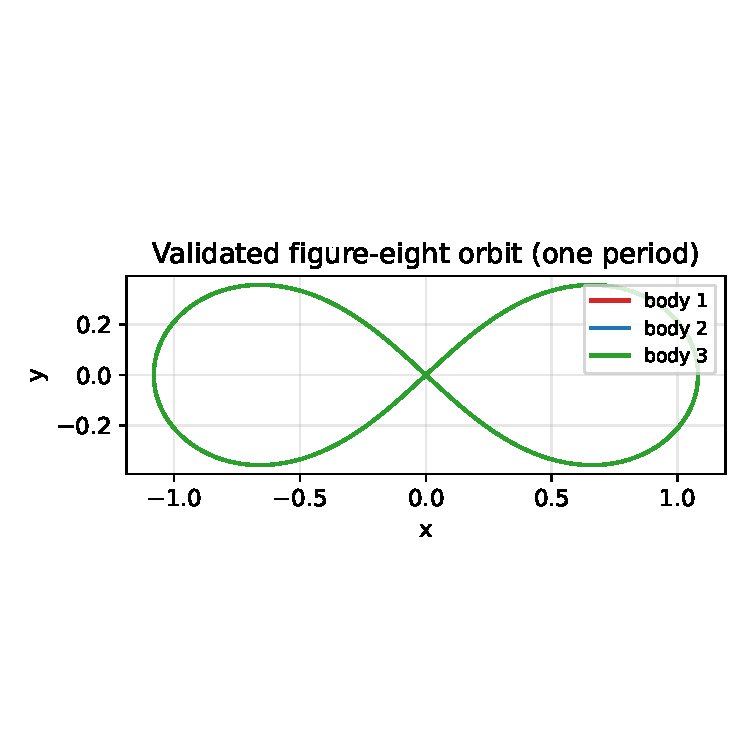
\includegraphics[width=0.55\textwidth]{fig_figure_eight.pdf}
  \caption{The figure-eight three-body orbit, independently refined and
    cross-checked in this project (orbit-closing error
    $2$--$4\times10^{-12}$, agreement between the two solvers
    $5.1\times10^{-12}$). \watch{\videoFigureEight}{animated version}.}
  \label{fig:figure8}
\end{figure}

% ======================================================================
\section{Q1: searching for new periodic orbits without a seed}
\label{sec:q1}
% ======================================================================

We tried four different searches for new periodic orbits. Each one was
built so that no already-known orbit is used to choose where to search or
what starting guess to try.

\subsection{Four searches}

\begin{enumerate}
  \item \textbf{Scanning the starting velocity's angle, along a line.}
    The three bodies start in a line
    ($\mathbf{r}_1=(-1,0)$, $\mathbf{r}_2=(1,0)$, $\mathbf{r}_3=(0,0)$),
    with zero total momentum, moving at some angle $\alpha$, and total
    energy fixed at $E=-1$ (this is always possible because gravity has
    no built-in length scale). We scanned $\alpha$ across $[0,\pi]$ in
    500 steps, looked for places where the orbit almost returns to its
    starting point, and refined the best candidates with a Nelder-Mead
    search followed by least-squares. Result: 21 candidates found, but
    none could be refined below an error of $10^{-7}$ (the best were
    between $0.2$ and $3.5$), and one trial run hit a genuine numerical
    singularity, later traced to an actual collision.
  \item \textbf{Starting at rest, in an isosceles triangle.} All three
    bodies start with zero velocity, with the third body at height $h$
    above the line joining the other two -- the classic construction due
    to H\'enon. When we removed the safety check that halts the
    simulation near a collision, \emph{every} value of $h$ we tried, from
    $0.15$ to $3.0$, ended in an actual collision within 1--2 time units.
  \item \textbf{Starting in a line, moving perpendicular to it.} All
    three bodies start in a line, moving perpendicular to it at some
    shared speed $v$. This whole family has exactly zero angular momentum
    no matter what $v$ is -- a direct result of the mirror symmetry built
    into the setup. At $v=0.1$, the two ``line-up'' events we detected, at
    $t=0.9934$ and $t=1.0050$, sit right on either side of $t=1.005$,
    which is exactly when an independent collision check says the bodies
    actually collided. These were not real, repeating alignments; they
    were numerical noise around an actual collision. Every value of $v$
    from $0.05$ to $1.2$ behaved the same way.
  \item \textbf{Scanning a genuine two-dimensional shape space.} The
    validated figure-eight orbit (Section~\ref{sec:figure8}) is
    \emph{not} in a line, even though it also has zero angular momentum.
    This suggested moving the third body off the line, to
    $\mathbf{r}_3=(0,h)$, and scanning both $\alpha$ and $h$ together: a
    $24\times24$ grid of 576 points at $E=-1$. We added a hard cutoff for
    any near-collision, plus an extra filter: any trial where two bodies
    ever came closer than $0.05$ to each other was thrown out before we
    even tried to refine it. 266 of the 576 grid points survived this
    filter. We took the 12 best survivors and refined them the same way
    as before. None converged below an error of $10^{-7}$; the closest we
    got was $0.93$.
\end{enumerate}

\subsection{What this means}

The first three searches show, with actual measured collision times, why
a naive line-shaped or zero-angular-momentum starting point is harder to
work with than it looks. Angular momentum normally acts like a barrier
that keeps three bodies from ever getting arbitrarily close together.
Without it, that barrier disappears, and a line-shaped starting point is
already sitting right next to the region where all three bodies collide.

The fourth search avoids this problem: it uses no known orbit to pick
where to search, only the general idea, borrowed from the figure-eight's
own shape, that moving off the line should help. It is clearly not
dominated by collisions, since more than half the grid survived our
filter. Even so, it did not find a new periodic orbit within the amount of
computing time we allowed.

So the honest answer to Q1, based on what we actually ran, is this: a
search built from symmetry alone, using no known orbit as a seed, did not
find a new periodic orbit within a reasonable computing budget. This fits
with, and helps explain, how much work the published discoveries actually
took. \citet{SuvakovDmitrasinovic2013} found 13 distinct new orbits out of
15 candidates using a similar shape-based search, but at a much larger
computational scale, and with an extra step we did not attempt:
classifying each candidate trajectory by the braid pattern -- essentially
a kind of knot -- it traces out, before ever trying to refine it.
\citet{LiLiao2017} later found 695 orbit families in total for equal
masses, more than 600 of them new, using an even larger search, and
\citet{LiJingLiao2018} found 1349 families (1223 new) for bodies of
unequal mass. Interestingly, that first Li \& Liao paper also found that
at least 7 of the original 15 Šuvakov-Dmitrašinović candidates lose their
periodicity once re-run at higher precision over long times -- a good
reminder that even published ``periodic'' orbits need the same kind of
double-checking we did in Section~\ref{sec:methods}.

In short, this is a negative result, but one with a clear, verified
cause. Zero angular momentum puts a search near the collision region, and
even once that region is avoided, a simple local search is not enough. It
likely takes either much more computing power or a smarter,
structure-aware search -- exactly what the published work used.

% ======================================================================
\section{Q2: building a solution that survives a chosen amount of time}
\label{sec:q2}
% ======================================================================

Unlike Q1, Q2 does not need an exactly periodic orbit, and it turns out to
have two separate, workable answers.

\subsection{Route 1: a direct construction for hierarchical systems}
\label{sec:q2-hierarchical}

A hierarchical triple -- a tight pair of bodies (1 and 2) orbited by a
third, distant body -- stays stable if the ratio of the outer orbit's size
to the inner orbit's size is above a threshold found by experiment. For a
flat, circular outer orbit, the Mardling \& Aarseth criterion
\cite{MardlingAarseth2001} is
\begin{equation}
  \frac{a_{\rm out}}{a_{\rm in}} \;\gtrsim\; 2.8\,
  \left[\frac{(1+q_{\rm out})(1+e_{\rm out})}{\sqrt{1-e_{\rm out}}}\right]^{2/5}
  \frac{1}{1-e_{\rm out}}
  \left(1 - \frac{0.3\,i}{180^\circ}\right),
  \qquad q_{\rm out} = \frac{m_3}{m_1+m_2},
  \label{eq:mardling}
\end{equation}
which, for equal masses, a circular outer orbit ($e_{\rm out}=0$), and no
tilt between the two orbits ($i=0$), works out to
$a_{\rm out}/a_{\rm in} \gtrsim 3.29$. An earlier version of our code left
out the $1/(1-e_{\rm out})$ factor. This did not change any number in this
paper, since every system here used a circular outer orbit, where that
factor equals exactly~1 -- but the corrected formula should be used for
any future work with an eccentric outer orbit.

We built three systems and ran each for 500 inner-orbit periods (2221
time units), using the validated scipy solver:

\begin{table}[htbp]
  \centering
  \begin{tabular}{lccc}
    \toprule
    $a_{\rm out}/a_{\rm in}$ & outcome & survived & energy drift \\
    \midrule
    6.0 (well above threshold) & stable & full 500 periods & $7.5\times10^{-10}$ \\
    3.3 (near threshold) & stable & full 500 periods & $4.2\times10^{-9}$ \\
    1.8 (below threshold) & disrupted & 18.1 periods & $2.2\times10^{-7}$ \\
    \bottomrule
  \end{tabular}
  \caption{Direct simulation checking the Mardling-Aarseth construction.}
  \label{tab:hierarchical}
\end{table}

\begin{figure}[htbp]
  \centering
  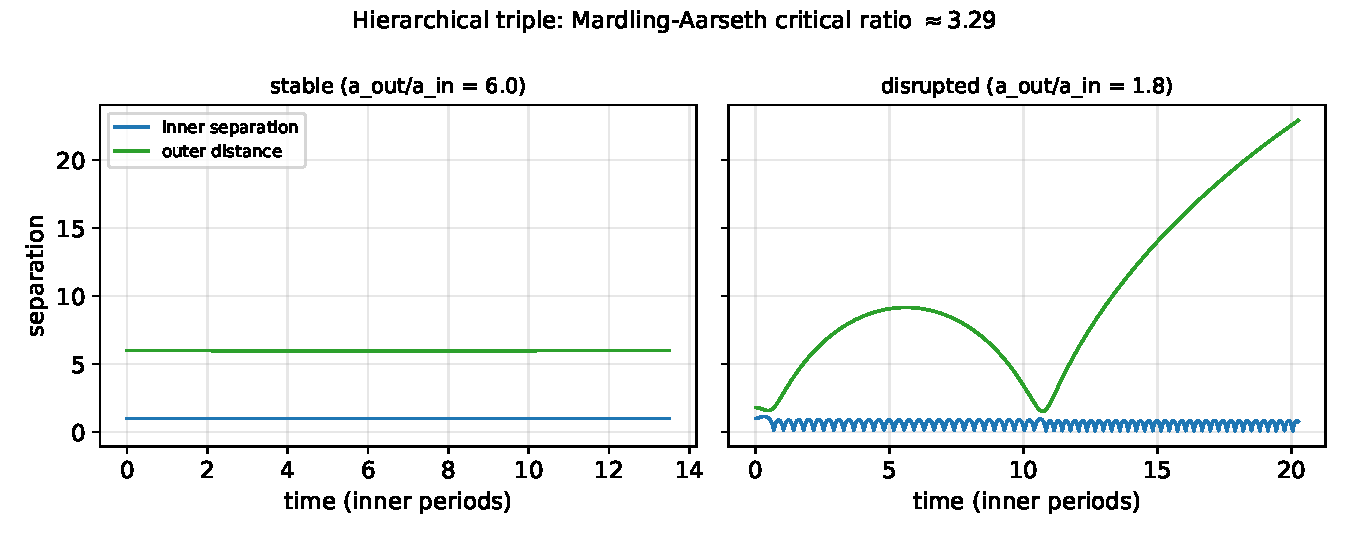
\includegraphics[width=0.9\textwidth]{fig_hierarchical.pdf}
  \caption{Inner-binary and outer-body separation vs.\ time (in inner
    periods) for a stable ($a_{\rm out}/a_{\rm in}=6.0$) and a disrupted
    ($a_{\rm out}/a_{\rm in}=1.8$) hierarchical triple.
    \watch{\videoHierarchical}{animated version}.}
  \label{fig:hierarchical}
\end{figure}

Given a target survival time $T$, measured in inner-orbit periods,
Eq.~\eqref{eq:mardling} tells us how wide to make the outer orbit. We then
confirmed by direct simulation that the resulting system really does
survive at least that long, with no trial-and-error search needed.

\subsection{Route 2: a survival curve for the typical, non-hierarchical case}
\label{sec:q2-statistical}

Most bound three-body systems are not hierarchical, so we also need an
answer for the general case. We generated 200 random three-body systems:
equal masses, zero total momentum, energy fixed at $E=-1$, with both the
shape and the direction of every velocity chosen at random. Unlike
Section~\ref{sec:q1}, we did \emph{not} force the angular momentum to
zero -- this is exactly what keeps most of these random systems away from
the collision region that caused so much trouble for Q1. Each system was
run until $t=200$, or until it either collided (any two bodies closer than
$10^{-3}$) or one body escaped (farther than 30 units from the center of
mass).

Out of 200 trials: 91 ended in collision (45.5\%), 82 ended in an escape
(41.0\%), and 27 (13.5\%) were still bound and intact at $t=200$. The
resulting survival curve, $S(T) = $ the fraction of trials still intact at
time $T$, is:

\begin{table}[htbp]
  \centering
  \begin{tabular}{lccccccccc}
    \toprule
    $T$ & 1 & 2 & 5 & 10 & 20 & 50 & 100 & 150 & 200 \\
    $S(T)$ & 0.965 & 0.945 & 0.910 & 0.865 & 0.770 & 0.540 & 0.295 & 0.180 & 0.135 \\
    \bottomrule
  \end{tabular}
  \caption{Fraction of 200 random trials surviving at least time $T$.}
  \label{tab:survival}
\end{table}

\begin{figure}[htbp]
  \centering
  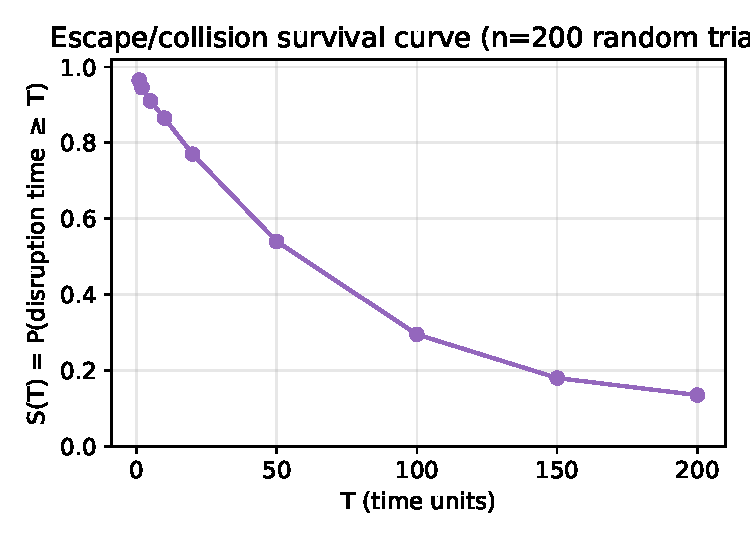
\includegraphics[width=0.5\textwidth]{fig_survival_curve.pdf}
  \caption{Survival curve for 200 random three-body scattering trials at
    $E=-1$. \watch{\videoSurvival}{animated version, with example
    collision and escape trajectories}.}
  \label{fig:survival}
\end{figure}

This answers Q2 for the typical, non-hierarchical case, but as a
probability rather than a guarantee. For any $T$ up to 200, $S(T)$ is both
the chance that a brand-new random system will survive that long, and it
comes with an actual example -- any of the 27 surviving trials -- that
does. That is a different kind of answer from Route~1. A random system
with unconstrained angular momentum has no structural protection, so its
chance of surviving falls off smoothly as $T$ grows, instead of the sharp
stable/unstable cutoff that Route~1's formula produces.
\citet{StoneLeigh2019} worked out a full statistical theory, based on the
assumption that this kind of chaotic breakup behaves ergodically, for
exactly this kind of outcome; our 200-trial curve is a small, direct
simulation in the same spirit, not a test of their specific formula.
\citet{Breen2020} later showed that a neural network trained on simulated
trajectories can make the same kind of prediction enormously faster -- a
way to speed up this statistical approach, not a third route.

% ======================================================================
\section{Visualizations}
% ======================================================================

Three Manim animations were produced directly from the numerical data
behind the figures above, not as stylized illustrations of a generic
three-body orbit:

\begin{itemize}
  \item \watch{\videoFigureEight}{Scene A}: the validated figure-eight
    orbit (Figure~\ref{fig:figure8}) over 2.5 periods, with a trail behind
    each body and a period counter.
  \item \watch{\videoHierarchical}{Scene B}: the stable
    ($a_{\rm out}/a_{\rm in}=6.0$) and disrupted ($a_{\rm out}/a_{\rm in}=1.8$)
    hierarchical triples from Section~\ref{sec:q2-hierarchical}, played
    at a common time scale so the difference in survival time is easy to
    see.
  \item \watch{\videoSurvival}{Scene C}: example collision and escape
    trajectories from the Section~\ref{sec:q2-statistical} experiment,
    together with the survival curve $S(T)$ as it grows.
\end{itemize}

% ======================================================================
\section{Conclusion}
% ======================================================================

A computer cannot solve the three-body problem in the sense of writing
down one formula that works for every case. But it can build and check
individual solutions to very high precision, and this paper's two
questions have different answers because they are really asking for
different things. Finding a brand-new, exactly periodic orbit (Q1) is
hard: all four of our from-scratch searches failed within a reasonable
computing budget, for a reason we could pin down directly. A simple,
symmetry-based search tends to land near the collision region, and even
once it avoids that region, it likely needs far more computing power or a
smarter, structure-aware search -- the kind used by
\citet{SuvakovDmitrasinovic2013} and by \citet{LiLiao2017}. Building a
system that merely \emph{survives} a chosen amount of time (Q2) is much
easier, and we found two separate ways to do it: a direct formula for
hierarchical systems that needs no search at all, and a statistical,
survival-curve approach for the general case. The taxonomy in
Section~\ref{sec:taxonomy} -- periodic vs.\ linearly stable vs.\
hierarchically stable vs.\ metastable -- is what makes this difference
between Q1 and Q2 precise, rather than just a matter of how the question
is phrased.

\bibliographystyle{plainnat}
\bibliography{references}

\end{document}
